\documentclass[14pt]{extbook}
\usepackage{multicol, enumerate, enumitem, hyperref, color, soul, setspace, parskip, fancyhdr} %General Packages
\usepackage{amssymb, amsthm, amsmath, latexsym, units, mathtools} %Math Packages
\everymath{\displaystyle} %All math in Display Style
% Packages with additional options
\usepackage[headsep=0.5cm,headheight=12pt, left=1 in,right= 1 in,top= 1 in,bottom= 1 in]{geometry}
\usepackage[usenames,dvipsnames]{xcolor}
\usepackage{dashrule}  % Package to use the command below to create lines between items
\newcommand{\litem}[1]{\item#1\hspace*{-1cm}\rule{\textwidth}{0.4pt}}
\pagestyle{fancy}
\lhead{Progress Quiz 6}
\chead{}
\rhead{Version B}
\lfoot{4563-7456}
\cfoot{}
\rfoot{Summer C 2021}
\begin{document}

\begin{enumerate}
\litem{
Construct the lowest-degree polynomial given the zeros below. Then, choose the intervals that contain the coefficients of the polynomial in the form $x^3+bx^2+cx+d$.\[ -5 + 5 i \text{ and } 3 \]\begin{enumerate}[label=\Alph*.]
\item \( b \in [-11, -3], c \in [16, 22], \text{ and } d \in [145, 151] \)
\item \( b \in [1, 6], c \in [-1, 7], \text{ and } d \in [-18, -13] \)
\item \( b \in [2, 12], c \in [16, 22], \text{ and } d \in [-156, -141] \)
\item \( b \in [1, 6], c \in [-9, 1], \text{ and } d \in [13, 20] \)
\item \( \text{None of the above.} \)

\end{enumerate} }
\litem{
Which of the following equations \textit{could} be of the graph presented below?
\begin{center}
    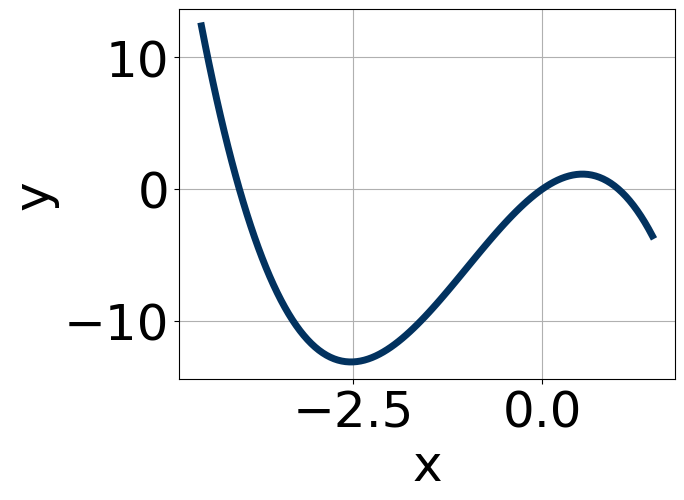
\includegraphics[width=0.5\textwidth]{../Figures/polyGraphToFunctionB.png}
\end{center}
\begin{enumerate}[label=\Alph*.]
\item \( -9x^{5} (x - 1)^{9} (x + 4)^{9} \)
\item \( 17x^{11} (x - 1)^{9} (x + 4)^{9} \)
\item \( 6x^{5} (x - 1)^{8} (x + 4)^{9} \)
\item \( -7x^{7} (x - 1)^{8} (x + 4)^{4} \)
\item \( -17x^{7} (x - 1)^{10} (x + 4)^{9} \)

\end{enumerate} }
\litem{
Which of the following equations \textit{could} be of the graph presented below?
\begin{center}
    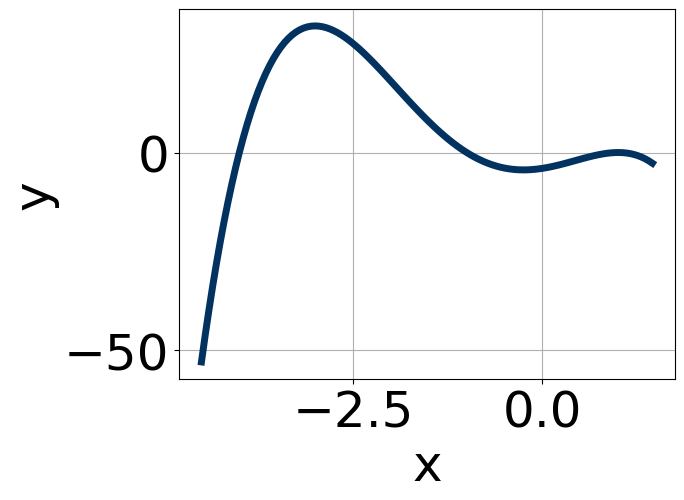
\includegraphics[width=0.5\textwidth]{../Figures/polyGraphToFunctionCopyB.png}
\end{center}
\begin{enumerate}[label=\Alph*.]
\item \( -17(x - 1)^{4} (x + 4)^{8} (x + 1)^{9} \)
\item \( 20(x - 1)^{10} (x + 4)^{7} (x + 1)^{4} \)
\item \( 2(x - 1)^{10} (x + 4)^{9} (x + 1)^{9} \)
\item \( -6(x - 1)^{7} (x + 4)^{8} (x + 1)^{11} \)
\item \( -4(x - 1)^{10} (x + 4)^{7} (x + 1)^{9} \)

\end{enumerate} }
\litem{
Describe the zero behavior of the zero $x = -6$ of the polynomial below.\[ f(x) = -4(x - 8)^{6}(x + 8)^{2}(x + 6)^{9}(x - 6)^{6} \]\begin{enumerate}[label=\Alph*.]
\begin{multicols}{2}\item 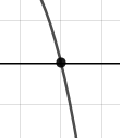
\includegraphics[width = 0.3\textwidth]{../Figures/polyZeroBehaviorCopyAB.png}\item 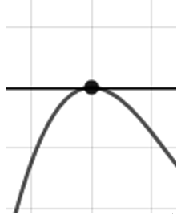
\includegraphics[width = 0.3\textwidth]{../Figures/polyZeroBehaviorCopyBB.png}\item 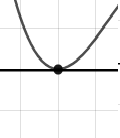
\includegraphics[width = 0.3\textwidth]{../Figures/polyZeroBehaviorCopyCB.png}\item 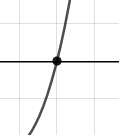
\includegraphics[width = 0.3\textwidth]{../Figures/polyZeroBehaviorCopyDB.png}\end{multicols}\item None of the above.
\end{enumerate} }
\litem{
Construct the lowest-degree polynomial given the zeros below. Then, choose the intervals that contain the coefficients of the polynomial in the form $x^3+bx^2+cx+d$.\[ -4 - 2 i \text{ and } -2 \]\begin{enumerate}[label=\Alph*.]
\item \( b \in [8, 13], c \in [34.2, 37], \text{ and } d \in [40, 42] \)
\item \( b \in [-4, 6], c \in [4.5, 8.2], \text{ and } d \in [6, 9] \)
\item \( b \in [-4, 6], c \in [3, 4.3], \text{ and } d \in [2, 5] \)
\item \( b \in [-14, -8], c \in [34.2, 37], \text{ and } d \in [-40, -32] \)
\item \( \text{None of the above.} \)

\end{enumerate} }
\litem{
Construct the lowest-degree polynomial given the zeros below. Then, choose the intervals that contain the coefficients of the polynomial in the form $ax^3+bx^2+cx+d$.\[ \frac{-7}{5}, \frac{5}{2}, \text{ and } \frac{-1}{4} \]\begin{enumerate}[label=\Alph*.]
\item \( a \in [35, 41], b \in [48, 58], c \in [-131, -125], \text{ and } d \in [-42, -32] \)
\item \( a \in [35, 41], b \in [-36, -27], c \in [-158, -150], \text{ and } d \in [33, 37] \)
\item \( a \in [35, 41], b \in [-148, -145], c \in [95, 106], \text{ and } d \in [33, 37] \)
\item \( a \in [35, 41], b \in [-36, -27], c \in [-158, -150], \text{ and } d \in [-42, -32] \)
\item \( a \in [35, 41], b \in [32, 40], c \in [-158, -150], \text{ and } d \in [33, 37] \)

\end{enumerate} }
\litem{
Describe the end behavior of the polynomial below.\[ f(x) = 8(x - 4)^{4}(x + 4)^{9}(x + 8)^{4}(x - 8)^{5} \]\begin{enumerate}[label=\Alph*.]
\begin{multicols}{2}\item 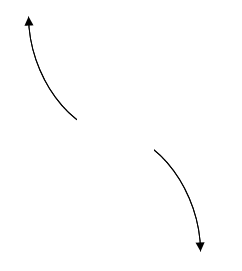
\includegraphics[width = 0.3\textwidth]{../Figures/polyEndBehaviorAB.png}\item 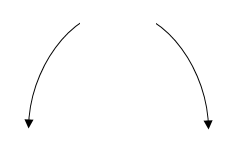
\includegraphics[width = 0.3\textwidth]{../Figures/polyEndBehaviorBB.png}\item 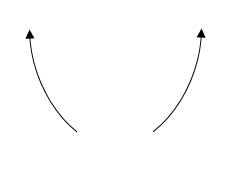
\includegraphics[width = 0.3\textwidth]{../Figures/polyEndBehaviorCB.png}\item 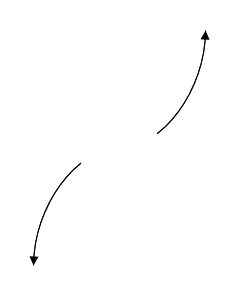
\includegraphics[width = 0.3\textwidth]{../Figures/polyEndBehaviorDB.png}\end{multicols}\item None of the above.
\end{enumerate} }
\litem{
Construct the lowest-degree polynomial given the zeros below. Then, choose the intervals that contain the coefficients of the polynomial in the form $ax^3+bx^2+cx+d$.\[ \frac{1}{2}, \frac{7}{4}, \text{ and } 4 \]\begin{enumerate}[label=\Alph*.]
\item \( a \in [7, 12], b \in [-23, -12], c \in [-71, -59], \text{ and } d \in [-32, -21] \)
\item \( a \in [7, 12], b \in [-51, -44], c \in [77, 82], \text{ and } d \in [-32, -21] \)
\item \( a \in [7, 12], b \in [49, 55], c \in [77, 82], \text{ and } d \in [28, 30] \)
\item \( a \in [7, 12], b \in [-51, -44], c \in [77, 82], \text{ and } d \in [28, 30] \)
\item \( a \in [7, 12], b \in [-44, -34], c \in [31, 43], \text{ and } d \in [28, 30] \)

\end{enumerate} }
\litem{
Describe the zero behavior of the zero $x = 2$ of the polynomial below.\[ f(x) = -4(x - 2)^{5}(x + 2)^{10}(x - 3)^{6}(x + 3)^{10} \]\begin{enumerate}[label=\Alph*.]
\begin{multicols}{2}\item 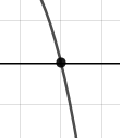
\includegraphics[width = 0.3\textwidth]{../Figures/polyZeroBehaviorAB.png}\item 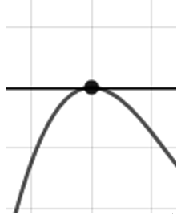
\includegraphics[width = 0.3\textwidth]{../Figures/polyZeroBehaviorBB.png}\item 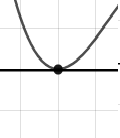
\includegraphics[width = 0.3\textwidth]{../Figures/polyZeroBehaviorCB.png}\item 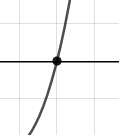
\includegraphics[width = 0.3\textwidth]{../Figures/polyZeroBehaviorDB.png}\end{multicols}\item None of the above.
\end{enumerate} }
\litem{
Describe the end behavior of the polynomial below.\[ f(x) = 2(x + 5)^{3}(x - 5)^{6}(x + 3)^{3}(x - 3)^{5} \]\begin{enumerate}[label=\Alph*.]
\begin{multicols}{2}\item 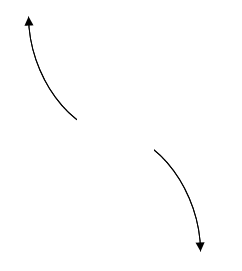
\includegraphics[width = 0.3\textwidth]{../Figures/polyEndBehaviorCopyAB.png}\item 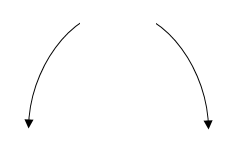
\includegraphics[width = 0.3\textwidth]{../Figures/polyEndBehaviorCopyBB.png}\item 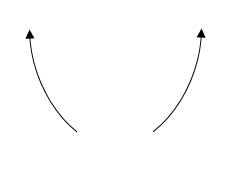
\includegraphics[width = 0.3\textwidth]{../Figures/polyEndBehaviorCopyCB.png}\item 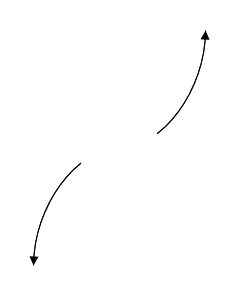
\includegraphics[width = 0.3\textwidth]{../Figures/polyEndBehaviorCopyDB.png}\end{multicols}\item None of the above.
\end{enumerate} }
\end{enumerate}

\end{document}